\section{Messwerte}

\begin{table}
  \centering
  \caption{gemessene Werte, Fallzeiten in s}
  \label{tab:Messdaten}
  \begin{tabular}{c c c c c }
    \toprule $Fallzeit \,\, Kugel \, 2 $ & $Fallzeit\,\, Kugel\, 1 $ &
             $Temperatur \,\, in \,\, \symup{°C}$ & $Messung \, 1 $ & $Messung \, 2$ \\
    \midrule
    11.80 & 68.47 & 31.0 & 68.86 & 68.86 \\
    11.80 & 68.95 & 36.0 & 68.33 & 68.21 \\
    12.15 & 68.69 & 39.0 & 65.75 & 65.76 \\
    11.73 & 68.53 & 45.0 & 60.32 & 60.52 \\
    12.21 & 68.50 & 49.5 & 59.27 & 59.27 \\
    11.47 & 67.69 & 51.5 & 58.52 & 58.66 \\
    12.10 & 68.83 & 56.0 & 58.30 & 58.29 \\
    11.96 & 68.41 & 60.0 & 56.60 & 56.72 \\
    11.86 & 68.38 & 64.0 & 55.10 & 55.15 \\
    11.87 & 68.60 & 68.0 & 54.35 & 54.40 \\
    \bottomrule
  \end{tabular}
\end{table}

\begin{table}
  \centering
  \caption{Mittelwerte der Fallzeiten in \texorpdfstring{$\symup{s}$}{b} für Teil 1 des Versuches}
  \begin{tabular}{c c c c}
    \toprule $Fallzeit \,\, Kugel \,\, 1$ & $\increment_{FK1}$ & $Fallzeit \,\, Kugel \,\, 2$ & $\increment_{FK2}$ \\
    \midrule
    68.50 & 0.30 & 11.89 & 0.13 \\
    \bottomrule
  \end{tabular}
  \label{tab:FallzeitenGemittelt}
\end{table}

\begin{table}
  \centering
  \caption{Mittelwerte der Messung bei verschiedenen Temperaturen für die große Kugel}
  \label{tab:TemperaturGemittelt}
  \begin{tabular}{c | c c c c c c c c c c }
    \toprule
    $Temperatur \,\, in \,\,\symup{K}$          & 304.15 & 309.15 & 312.15 & 318.15 & 322.65 \\
    $Fallzeit \,\, in \,\,\symup{s}$            & 68.86 & 68.27 & 65.76 & 60.42 & 59.27 \\
    $\increment_{FZ} \,\, in \,\,\symup{s}$     & 0 & 0.035 & 0.002 & 0.058 & 0 \\
    \midrule
    $Temperatur \,\, in \,\, \symup{K}$          & 324.65 & 329.15 & 333.15 & 337.15 & 341.15 \\
    $Fallzeit \,\, in \,\, \symup{s}$           & 58.59 & 58.29 & 56.66 & 55.13 & 54.38 \\
    $\increment_{FZ} \,\, in \,\, \symup{s}$     & 0.040 & 0.003 & 0.035 & 0.014 & 0.014 \\
    \bottomrule
  \end{tabular}
\end{table}

\newpage

\section{Auswertung}

\subsection{Bestimmung der Apparatekonstante für die große Kugel}

In dem ersten Teil des Versuches soll die Apparatekonstante für die große Kugel (Kugel 1) bestimmt
werden. Dafür wird mithilfe der bekannten Apparatekonstante für die kleine Kugel (Kugel 2) die Viskosität
des Wassers bei Raumtemperatur bstimmt und in folgende Formel eingesetzt:

\begin{align}
  \label{eqn:KappaGroß}
  \Kappa_{kl} &= 0.007640 \, \symup{mPa\, cm^3 / g} \\
  \eta        &= \Kappa_{gr} \cdot \left( \rho_K - \rho_{Fl} \right) \cdot t
\end{align}

Bei $\rho_K$ und $\rho_{Fl}$ handelt es sich um die Dichten der Kugel und der betrachteten
Flüssigkeit. Mithilfe der gemessenen Radien und Gewichte der Kugeln kann die Dichte
bestimmt werden:

\begin{align}
  r_{gr}    &= (0.0078017 \pm 0.0000017) \, \symup{m}     & r_{kl}    &= (0.0077167 \pm 0.0000017) \, \symup{m} \\
  m_{gr}    &= 0.00496 \, \symup{kg}                        & m_{kl}    &= 0.00446 \, \symup{kg} \\
  \rho_{gr} &= (2493.6 \pm 1.6) \, \symup{kg/m^3} & \rho_{gr} &= (2312.0 \pm 1.5) \, \symup{kg/m^3}
  \label{eqn:Daten}
\end{align}

In Tabelle \ref{tab:FallzeitenGemittelt} sind die Mittelwerte und Fehler der gemessenen Fallzeiten für die
kleine und Große Kugel bei Raumtemperatur eingetragen.
Somit ergeben sich für die Viskosität des Wassers bei Raumtemperatur $\eta_{20}$ und $K_{gr}$ folgende Werte:

\begin{align}
  \eta_{20}   &= (0.001194 \pm 0.00013) \, \symup{Pa \, s} \\
  \Kappa_{gr} &= \frac{\eta_{20}}{\left( \rho_{gr} - \rho_{w} \right) \cdot t_{gr}} \\
              &= (0.001165 \pm, 0.00012) \, \symup{mPa\, cm^3 / g}
\end{align}

Die Fehler für $\eta_{20}$ und $\Kappa_{gr}$ ergeben sich mit der Gaußschen Fehlerfortpflanzung:

\begin{align}
\increment \eta    &= \sqrt{ \left( \partial_{\rho_{gr}} \eta \cdot \increment \rho_{gr} \right)^2 + \left( \partial_{t_{gr}} \eta \cdot \increment t_{gr} \right)^2  }\\
\increment K_{gr} &= \sqrt{ \left( \partial_{\eta} K_{gr} \cdot \increment \eta \right)^2 + \left( \partial_{\rho_{gr}} K_{gr} \cdot \increment \rho_{gr} \right)^2 +
                      \left( \partial_{t_{gr}} K_{gr} \cdot \increment t_{gr} \right)^2  }
\end{align}

\begin{figure}
  \centering
  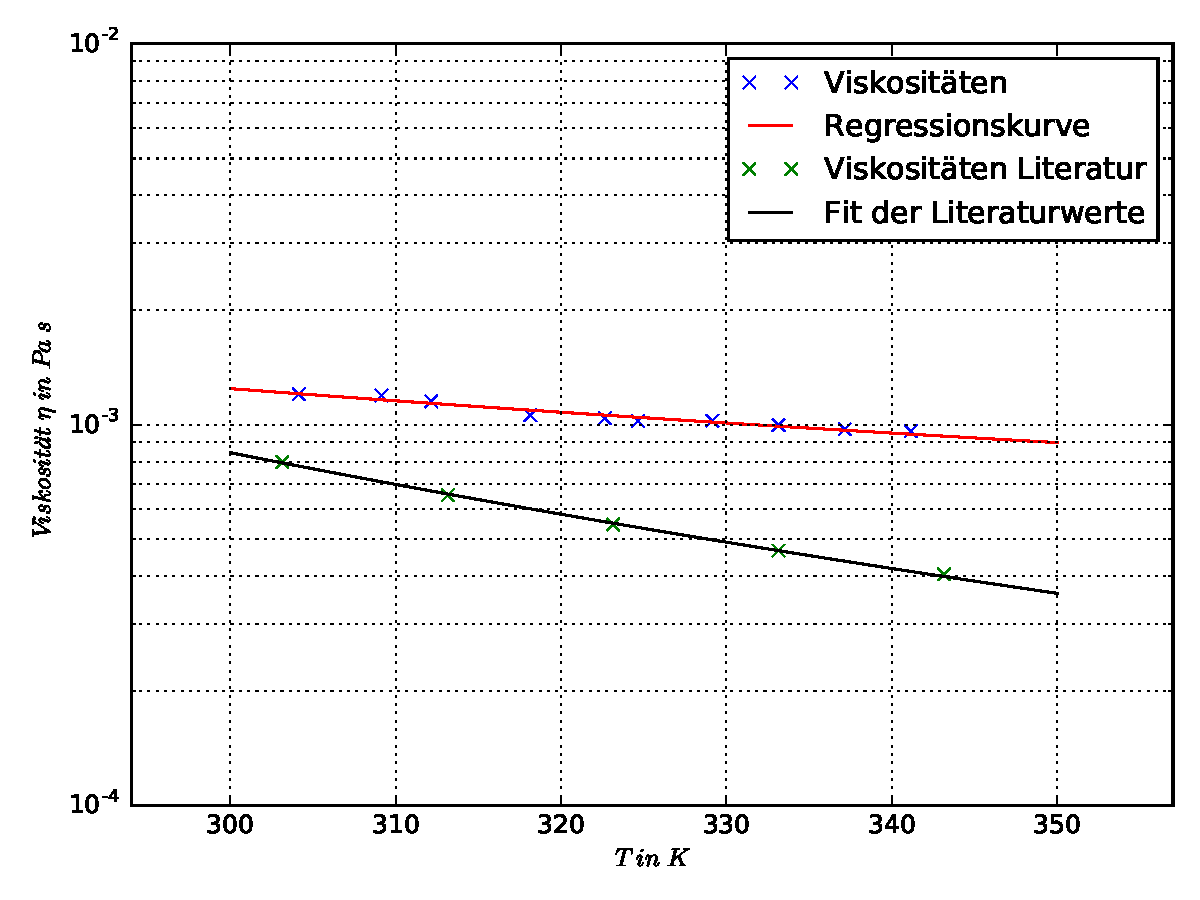
\includegraphics[height = 9.2 cm]{Plot_T.pdf}
  \caption{Viskositäten gegen T}
  \label{plt:ViskosT}
\end{figure}

\begin{figure}
  \centering
  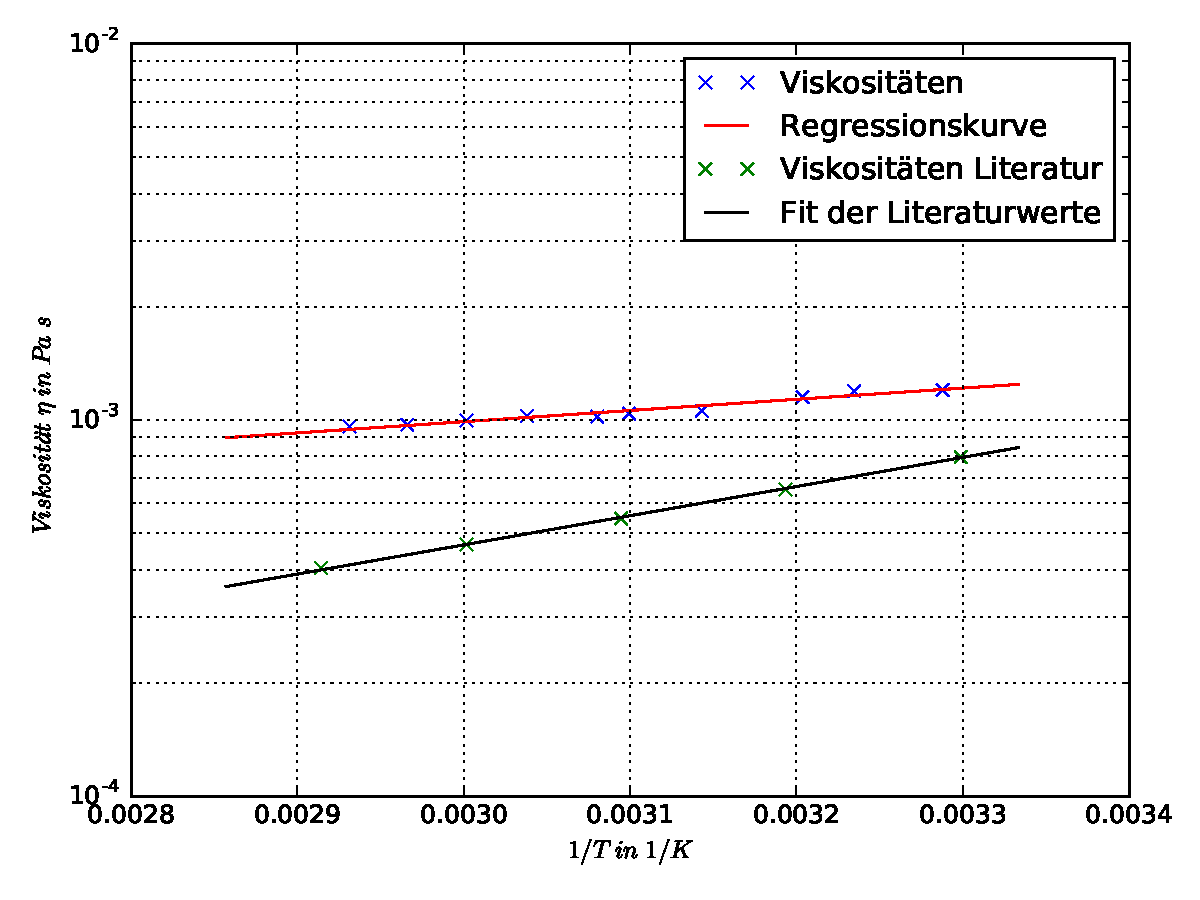
\includegraphics[height = 9.2 cm]{Plot_T_1.pdf}
  \caption{Viskositäten gegen 1/T}
  \label{plt:Viskos_T}
\end{figure}

\subsection{Bestimmung der Konstanten A/B für die zeitabhängige Viskosität \texorpdfstring{$\eta(T)$}{z}}

In den beiden Abbildungen \ref{plt:ViskosT} und \ref{plt:Viskos_T} sieht man einmal die Viskosität gegen T und einmal gegen 1/T aufgetragen.
Zum Vergleich sind in beiden Graphen auch die Literaturwerte mit eingebunden.
Die y - Skala ist dabei logarithmisch angepasst. Die Plots wurden mithilfe von Python erstellt und ergeben
für A und B folgende Parameter:

\begin{align}
  \symup{A} &= 1.2651 \cdot 10^{-4} \\
  \symup{B} &= 6.8567 \cdot 10^{2}
\end{align}

Somit ergibt sich für die Andradesche Gleichung für die Temperaturabhängigkeit der Viskosität von destilliertem
Wasser folgende Formel:

\begin{equation}
  \eta(\symup{T}) = 1.2651 \cdot 10^{-4} \cdot \exp \left( \frac{6.8567 \cdot 10^{2}}{\symup{T}} \right)
\end{equation}

\subsection{Bestimmung der Reynoldszahl}

Mithilfe der Formel für die Reynoldszahl \eqref{eqn:Reynolds Zahl} kann bei dem vorliegenden Versuch beurteilt werden, ob es
sich um eine laminare Strömung handelt. Als kritische Zahl für Rohrströmungen gilt normalerweise ein Faktor
von ca. 2300. Da für das $d$ in diesem
Fall jedoch nicht der Querschnitt der Strömung, sondern der Durchmesser der umströmten Kugel verwendet wird,
halbiert sich dieser Wert zu $Re_{krit} = 1150$.

Die Geschwindigkeit der Kugel für die verschiedenen Temperaturen lassen sich mit den gemessenen Fallzeiten in
Tabelle \ref{tab:TemperaturGemittelt} und der vorher bekannten Messtrecke von $S = 0.1$ m berechnen. Sie sind
in der folgenden Tabelle eingetragen.

\begin{table}
  \centering
  \caption{Geschwindigkeit der großen Kugel für verschiedene Geschwindigkeiten}
  \label{tab:Geschwindigkeiten}
  \begin{tabular}{c | c c c c c }
    \toprule
    $v \,\, in \,\,  \frac{m}{s} $ & 0.145 & 0.146 & 0.152 & 0.166 & 0.169 \\
    $\increment v \,\, in \,\,  \frac{m}{s} \cdot 10^{-5} $ & $0$ & $7.432$ & $0.667$ & $15.81$ & $0$ \\
    \midrule
    $v \,\, in \,\,  \frac{m}{s} $ & 0.171 & 0.172 & 0.176 & 0.181 & 0.184 \\
    $\increment v \,\, in \,\,  \frac{m}{s} \cdot 10^{-5} $ & $11.77$ & $0.849$ & $10.79$ & $4.749$ & $4.882$ \\
    \bottomrule
  \end{tabular}
\end{table}

\newpage

Mit dem in \eqref{eqn:Daten} angegebenen Radius der Kugel und der Dichte von Wasser für die jeweiligen
Temperaturen ergeben sich für die Reynoldzahlen nun folgende Werte:

\begin{table}
  \caption{Reynoldszahlen für die verschiedenen Temperaturen}
  \label{tab:Reynolds}
  \begin{tabular}{c | c c c c c c c c c c }
    \toprule
    $Temperatur \,\, in \,\, \symup{°C}$ & 31 & 36 & 9 & 45 & 49.5 & 51.5 & 56 & 60 & 64 & 68 \\
    \midrule
    $Re$                            & 18.8 & 19.0 & 20.5 & 24.2 & 25.0 & 26.0 & 25.8 & 27.1 & 28.6 & 29.2 \\
    $\increment Re $                & 0.2 & 0.2 & 0.2 & 0.3 & 0.3 & 0.3 & 0.3 & 0.3 & 0.3 & 0.3 \\
    \bottomrule
  \end{tabular}
\end{table}

\section{Auswertung}

Wie man in den Abbildungen \ref{plt:ViskosT} und \ref{plt:Viskos_T} erkennen kann, weichen die
ermittelten Viskositäten für destilliertes Wasser deutlich von den Literaturwerten ab. Durch einen
Fit der Literaturwerte an die Andradesche Gleichung ergeben sich die Parameter $ A = 2.19 \cdot 10^{-6} $
und $ B = 1.79 \cdot 10^{3} $. Im Durchschnitt weichen die Funktionen um ca. $ 0.000495 \, \symup{Pa \, s}$ ab.
Jedoch ist auch erkennbar, dass das Verhalten beider Funktionen sich ähnelt, somit kann ein systematischer Fehler
bei diesem Experiment wohl ausgeschlossen werden.

Die ermittelten Reynoldszahlen lassen sich schlecht mit Literaturwerten vergleichen, da sie für jedes Experiment aufgrund
der Abhängigkeiten von Apparaturwerten unterschiedlich sind. Allerdings sind die ermittelten Reynoldszahlen deutlich
kleiner als der in Abschnit 4.2 angegebene kritische Wert $R_{krit} = 1150$. Somit handelt es sich mit einer ziemlich
großen Sicherheit bei dem beobachteten Experiment um laminare Strömungen.

Die entstandenen Abweichungen für die Viskositäten sind vermutlich auf statistischen Fehler zurückzuführen. Ein
großer Faktor war vermutlich die Zeitmessung bei dem Experiment. Hier ist einerseits die menschliche Reaktionszeit
mit einzubeziehen und andererseist ist die gemessenen Zeiten auch davon abhängen, ob man beim Start und Ende jeder Messung
jeweils den selben Referenzpunkt der Kugel beobachtet, was in der Praxis schwer exakt zu realisieren ist.
